

\begin{figure}[h]
\centering
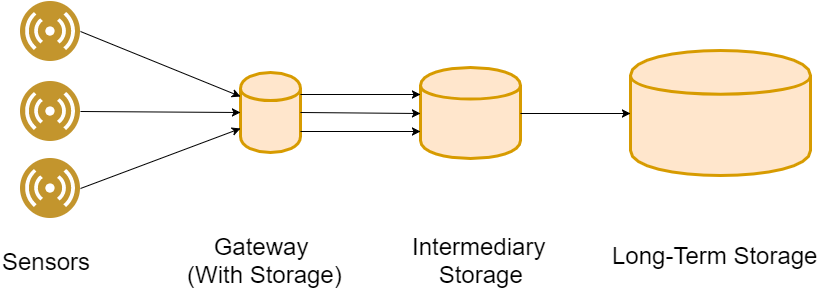
\includegraphics[width=\textwidth]{figures/pipeline.png}\\
\caption{Pipeline architecture}
\label{pipeline}
\end{figure}
The following section provides details on the design and implementation of the proposed IoT data delivery pipeline. 

In the context of a smart grid it is common to have a setup in which sensors are not directly connected to a data center to deliver the generated sensor data but connected to a gateway, that is close to the site of where the sensors are deployed. Also the gateway can then be connected to another intermediary hop, forming a so called "pipeline" to deliver the data to the data center. In such a scenario a sensor will send its measurements to the first gateway of the pipeline. The gateway will receive the message, maybe perform transformations to the data like aggregation, and forward the measurements to the next intermediary node in the pipeline. The intermediary node might also transform the data and forward it to the next hop. This process will repeat until the endpoint of the pipeline, the data center, will be reached. 

For that reason an implementation for such a pipeline has to be applicable not only to be run in data center but also on devices with limited resources available. This generates requirements like, being able to run on limited resources, as well as also performing well on limited resources. More over limitations in bandwidth, of the links between the different gateways in the pipeline should be considered.
Figure \ref{pipeline} provides an overview on the given pipeline architecture. Moreover should the gateways and intermediary nodes provide a suitable amount of storage to be able to deal with outages of a subset of the nodes in the smart grid. This should prevent data loss in a big scale and ensure that the pipeline and especially the smart grid, can remain operational in case of any partial outages. For that purpose also different and limited storage capabilities have to be taken into account when designing and choosing the database for the different types of nodes throughout the pipeline. The following will therefore provide a description of the technologies that are used for the first prototype implementation to meet all the different requirements and provide a description on how the components are implemented.


\subsection{gRPC}
GRPC is an open source remote procedure call(RPC) framework, that is built on top of HTTP2 connections and using Google Protocol Buffers for serializing the data that is transmitted and as interface description language. It provides an abstraction of the interfaces that have to be implemented and enables users to use different programming languages to implement their services. Many popular programming languages are supported, like Python, Java and C++. It also supports different platforms and can run in different environments, including data centers but also smaller and mobile devices. In addition to the afore mentioned gRPC provides support for bi-directional and client streaming RPCs and promises high performance. All the mentioned points make gRPC a suitable framework to choose for our pipeline implementation, since it promises to provide high performance in terms of throughput as well as latency, ease of use to the support of many different programming languages and the use of Google protocol buffers. The following section describes Google protocol buffers in general, how the developed message protocol for the pipeline implementation looks like and how the services are defined.
\subsubsection{Google Protocol Buffers}
 Google Protocol Buffers are a language and platform independent method to serialize structured data and generate the needed code for many different programming languages. It supports Python, Java, C++ and others. The message format has to be defined in a .proto file following the Protocol Buffer Language. After the .proto file is created, the code in the desired language can be generated. Google Protocol Buffers promise to be fast and small in size, and compared to XML offer 20 to 100 times faster serialization and 3 to 10 times less size.
 The following will provide an overview on how the developed message format for the given task looks like.

\subsubsection{Message Format}
In order to be able to make use of the sensory data for the services needed to be deveolped for the given task, a message format had to be designed. The available parameters generated by each sensor in the smart grid was given. These parameters are: 
\begin{itemize}
\item Meter ID, an unique ID of a sensor
\item Metric ID, an unique ID to define the metric of a value
\item Timestamp, a timestamp with the time the sensor value got created
\item Value, a sensor measurement value
\end{itemize}
To reflect the parameters generated by the sensors, the measurement message format is created in the .proto file as follows:
\begin{lstlisting}
message measurement_message {
  string meter_id = 1;
  string metric_id = 2;
  int64 timestamp = 3;
  double value = 4;
}
\end{lstlisting}
With that all the needed parameters generated by a sensor are reflected in our message format. In addition to that two further parameters are needed, taking the proposed Provenance API into account. The additional parameters are:
\begin{itemize}
\item Provenance ID, an unique ID to identify a specific provenance datapoint
\item Context Parameters, a string containing all enabled context parameters 
\end{itemize}
To reflect these parameters as well, the following message format was created:
\begin{lstlisting}
message Grid_data {
  measurement_message measurement = 1;
  string prov_id = 2;
  string context = 3;
}
\end{lstlisting}
So the Grid\_data message contains a message following the measurement\_message format and the needed parameters for the Provenance API. Note that each field in the message is optional by default, so not every field in a message have to set.
In addition to the messages defined, a reply message was defined, that only contains a response code that follows common HTTP Status codes.
\begin{lstlisting}
message reply {
  string response_code=1;
}
\end{lstlisting}
With the defined messages, all the needed parameters originating from the sensors and the parameters of the Provenance API can be reflected.

\subsubsection{gRPC Service Definition}
In addition to the message format, a service definition, so an interface for the pipeline components has to be defined. To provide a preferably adaptable interface for all types of gateways between the sensors and the Long-Term Storage, one service was defined as follows.
\begin{lstlisting}
service gateway {
  rpc push_data(stream Grid_data) returns (reply) {}
}
\end{lstlisting}
With that the gateway service is defined, which exposes one RPC called push\_data. The push\_data RPC expects an input stream of messages of type Grid\_data and responds with a message with type reply. This means that the service is receiving a stream of messages, so several messages of type Grid\_data at once. The decision to implement it in this way was made due to the fact that otherwise the reply would have to be sent after each received message, which in return would increase network overhead. The benefit of using gRPC for the definition of the message format and the interface is that with the defined .proto file, the needed serialization code and code stubs to implement the RPC service can be generated in the programming language one desires. It was also the basis for the sensor data emulator described in the following section.

\subsubsection{Sensor data emulator(Dominik)}
Based on the already described message format and the service definition, we were provided with an emulator to simulate the generation of sensory data. It was used to simulate the sensors in a pipeline scenario.

\subsection{Local Storage}
As already mentioned, a way to store measurement messages on each node of the pipeline locally, is needed. The chosen database has to be able to run on all the different types of nodes, so it has to be able to run on smaller and less powerful gateway nodes and more performance offering nodes as small servers or in data centers. More over it has to provide a high write performance to be able to deal with a high load of receiving messages and therefore write operations. It also has to be scalable, lightweight and quick to respond. In addition to that and to be able to deal with the use case specific problem of outages in a smart grid, the database also has to offer persistent storage.  
\subsubsection{Redis}
Taking into account the data model of a measurement message, the decision was made to use a key-value storage database. In addition to that all the listed requirements have to be met, and especially keeping in mind the need for a database coping with different hardware configurations, the key-value in-memory database Redis was finalized as database to be used.
Redis meets all the requirements such as high performance on write operations. Even though it is an in-memory database it also provides the possibility of being persistent. Snapshots and write operation logs, can be used to provide persistence. 

The following section will provide an overview on the implementation and explains the most important parts of it in detail.
\subsection{Implementation}

\begin{figure}[h]
\centering
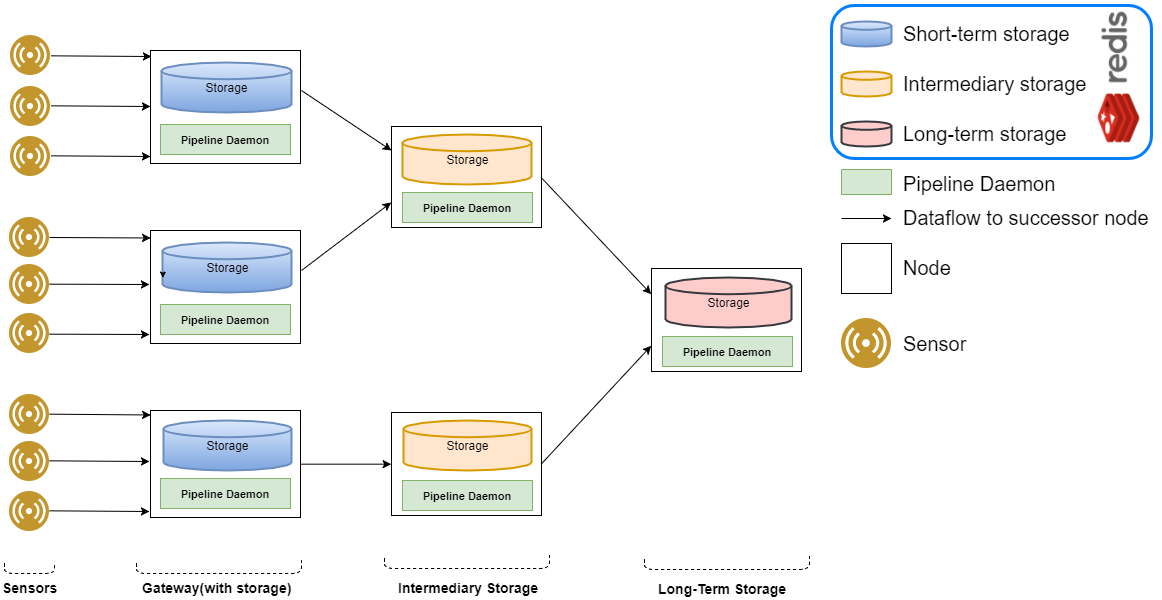
\includegraphics[width=\linewidth]{figures/pipelinearchitecture.png}\\
\caption{Pipeline architecture}
\label{pipeline_arch}
\end{figure}
In this section a detailed description and explanation of the pipeline implementation is presented. The pipeline is implemented in the programming language Java. For the build management, Apache Maven is used. The Java project is organized as follows. The code for the pipeline component resides in the PipelineComponent class. In addition to that the PipelineInterfaces.proto file provides the already described service and message definitions used to generate the serialization and service stub code. 

First of all, the system architecture is visualized in figure \ref{pipeline_arch}. One node in the pipeline consists of a database to provide local storage and a Pipeline Daemon.
The Pipeline Daemon is used to implement the already described service gateway.

\subsubsection{Pipeline Daemon}
The generated gRPC code was used to implement the gateway service and its RPC push\_data. The different types of nodes, that can be part of the pipeline, can be created when starting a component, by the use of different run configurations. A Pipeline Daemon can either be run as a gateway or as an endpoint. For that purpose a set of configuration parameters are provided. The following parameters are available:
\begin{itemize}
\item port, the port used by the server of this Daemon
\item port\_next, the port of the next hop in the pipeline
\item host\_next, the hostname or IP of the next hop in the pipeline
\item location, a label for the current physical location of the node
\item storageTime, an integer value representing the time messages are stored in seconds
\item propertiesfile, specifying the path to the Provenance Daemons properties file 
\item no\_prov, flag that can be set to turn of the collection of provenance data and the use of the provenance system
\end{itemize}
If the parameters host\_next and port\_next are set, the Pipeline Daemon is recognized as a gateway. On the other hand if these parameters would not have been set, the Pipeline Daemon is recognized as endpoint of the pipeline, since there is no successor. In addition to implementing the service gateway, the Pipeline Daemon implements a client, based on the push\_data interface definition, to be able to make use of the gateway services of other components in the pipeline. This is the case if the Pipeline Daemon is started as gateway. Then it has to be able to receive the messages from another clients and forward them to the next hop in the pipeline. 

The gateway service provides the push\_data service, as mentioned. The push\_data service is responsible of processing the messages a client sent. The client can send messages one by one, or send them as a stream of messages, so the client can send many messages at once. If the client sends a message and the push\_data service is called, it will process the message. The push\_data service is responsible for collecting the needed context information to feed to the Provenance Daemon and provide information, e.g. how many messages are received and sent per second. In case of receiving a stream of messages the push\_data service will cache the received messages and the generated context information. If the stream exceeds the number of 10 messages, the cached context information will be already forwarded to the Provenance Daemon and the measurement messages will be sent to the next hop, while still receiving the stream of messages. If the stream the client sends contains less then 10 messages, the push\_data service waits for the stream to be finished, before forwarding the context information to the Provenance Daemon and forwarding the messages to the next hop in the pipeline. This behavior was implemented due to the fact, that it is possible to use one single stream to send a large number of messages. If the Pipeline Daemon would wait until all messages arrived it is possible that additional delay is introduced and the latency increases. More over it would also result in irregular peak workload on the network, which is prevented when splitting up the incoming stream.   

Additionally there is the possibility that the no\_prov flag was set on startup of the Pipeline Daemon. In this case the push\_data service will not collect any context information. It will just cache and forward the measurement messages. 
The behavior of caching messages if the stream exceeds the number of 10 messages, remains the same. More over the provenance daemon will not be instantiated.

For the purpose of providing information like the number of messages per second to the developed user interface and to capture the health of the pipeline component daemon, additional methods are implemented by the push\_data service. A counter in combination with a timer is used to capture the number of messages. The advertisement of the values to the user interface is handled by the Provenance API. The node health is for one implicitly set when interacting with the provenance API, and for the other it is set by the use of a timer if the push\_data services is not interacting with the Provenance API.

\subsubsection{Local Storage}
For the use of the local storage, so the Redis database, a Redis client is implemented with the Pipeline Daemon. The push\_data service will, while processing the messages, save the measurement messages in the local Redis database. If the Provenance Daemon is active the Provenance IDs, that are received after the created context datapoints are handed to the Provenance Daemon, will be used as the keys for the measurement messages. This will also ensure, that in case of a failure the original messages can be retrieved from the local database and linked to the provenance entries in the Provenance DB. In contrast to that the current system time in nanoseconds is used if the no\_prov flag has been set. The measurement messages are saved as hashes, so with one key a whole measurement message can be saved.

The implementation of a Pipeline Daemon and the gateway service that is used for all different types of nodes, remains the same. From service implementation point of view it will only be differentiated between gateways and endpoints of the pipeline, so if messages will be forwarded to another hop in the pipeline or not. Only the amount of local storage provides a differentiation between different nodes. To be able to reflect this in the implementation, the storageTime configuration parameter is used. The parameter is used to simulate the different amount of storage available on the different machines that are part of the pipeline. A timer is used along with the specified time of the storageTime parameter so that after the timer expires the database will be flushed. With this it is ensured to reflect different storage capabilities with the Pipeline Daemon prototype implementation.






